\chapter{Namens- und Verzeichnisdienste}

\section{Namensdients}
Ein \textbf{Namensdienst} bildet einen (menschenfreundlichen) Namen zu einem Objekt ab. Beispielsweise assoziiert das Dateisystem einen Dateinamen zu einem \emph{Filehandler} und der DNS einen Namen zu einer IP-Adresse. Das \textbf{Namenssystem} beschreibt den Syntax, welcher für die Namen befolgt werden muss. Das Unix-Dateisystem schreibt vor, dass der Name immer mit einem '/' beginne muss (/etc/hosts). Im DNS werden Objekte mit dem Punkt-Operator (www.20min.ch) deklariert. Der Assoziations-Vorgang zwischen Namen und Objekt wird \textbf{binding} genannt. Typischen Namensdienste: RMI Registry, CORBA Naming Service.

\section{Verzeichnisdienst}
Der \textbf{Verzeichnisdienst} kann im Gegensatz zu einem reinen Namensdienst etwas mehr. Es werden nicht nur Bindings erstellt, sondern es können auch Verzeichnisdienst spezifische Attribute zum Objekt abgelegt werden. Auf Basis diesen Attributen kann im Verzeichnis gesucht werden. Typischer Verzeichnisdienst: LDAP.

\section{JNDI}
Das Java Naming und Directory Interface (JNDI) ist ein Java-API für Namens- und Verzeichnisdienste. Über die Schnittstelle können Daten- und Objektreferenzen anhand eines Namens abgelegt und von Nutzern des API wieder abgerufen werden. Dieses API ist ein sogenanntes Server Provider Interface (SPI), damit können Hersteller eigene Lösungen bauen. Über JNDI werden die meisten bekannten Dienste unterstützt, wie: LDAP, DNS, NIS (Network Information Service), CORBA (Common Object Request Broker Architecture), Dateisystem, RMI. Wir dürfen froh sein, dass wir mit EJB 3.x arbeiten. Davor mussten alle Referenzen auf Ressourcen im Deployment Deskriptor verwaltet werden und anschliessend mittels JNDI-Lookups in den EJBs programmiert werden. Es gab weder Annotationen noch die mächtigen Mechanismen der Dependency Injection.

\subsection{API}
Das API beinhaltet folgendes:
\begin{itemize}
	\item Mechanismus zum Binden von Objekten an einen Namen
	\item Methoden für den Abruf von Informationen anhand eines Namens
	\item Clients können über Änderungen informiert werden, dies ist mittels einem Ereigniskonzept umgesetzt
	\item Spezielle Erweiterungen für LDAP-Funktionalitäten
\end{itemize}

\subsection{Architektur}
Am einen Ende ist das JNDI und am anderen Ende die Server Provider Implementation, welche über das Service Provider Interface spezifiziert ist. Der Naming-Manager ist das Verbindungsstück zwischen API und SPI.

\begin{figure}[h!]
\centering
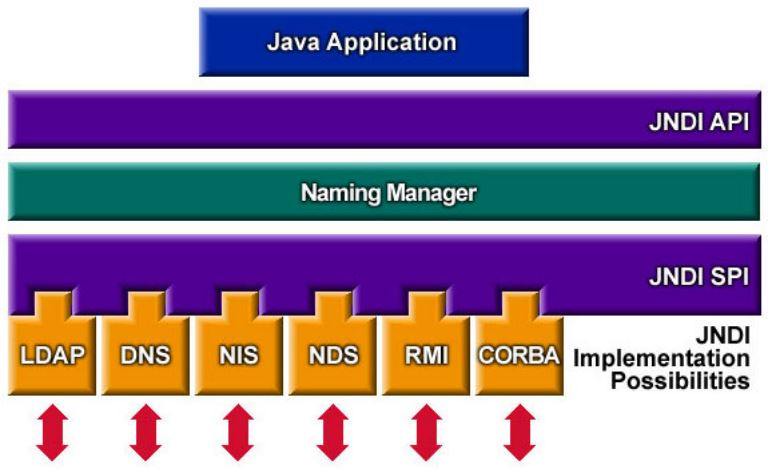
\includegraphics[width=0.5\linewidth]{fig/jndi-architecture}
\caption{JNDI Architektur}
\label{fig:jndi-architecture}
\end{figure}

\subsection{Packages}
\begin{description}
	\item[javax.naming:] Definiert ein Naming Context Interface, welches
	das Core-Interface für lookups, bind/unbind, renaming für
	Objekte und erzeugen/löschen von Subkontext darstellt.
	\item[javax.naming.directory:] Erweitert das Naming-Package mit den
	Zugriffen auf Namens Services. Erlaubt das Abholen von
	Attributen assoziert mit Objekten gespeichert im Directory.
	\item[javax.naming.event:] Unterstützt die Event Notifikation in
	Directory Services. Es gibt Events und Listeners.
	\item[javax.naming.ldap:] Erweitert das javax.naming.directory Packet
	mit erweiterten Operation Controls. Auf Basis von LDAPv3.
	\item[javax.naming.spi:] Unterstützt die Entwickler von
	Namensdiensten bei der Implementierung von Services. 
\end{description}

\subsection{JNDI-Lookup}
Beim \textbf{Lookup} (Nachschlagen) wird den Name verwendet um das korrespondierende Objekt zu ermitteln. 

\begin{lstlisting}[language=Java, caption=Beispiel programmatischer EJB-Lookup]
try {
	Friend friend = (Friend) new InitialContext().lookup("java:comp/env/myFriend");
} catch (NamingException e) {
	e.printStackTrace();
}
\end{lstlisting}

\begin{figure}[h!]
\centering
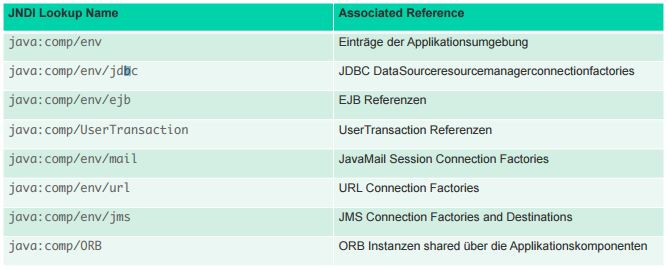
\includegraphics[width=0.7\linewidth]{fig/jndi-lookups}
\caption{JNDI Lookups und assoziierte Referenzen}
\label{fig:jndi-lookups}
\end{figure}

\subsection{Externe JNDI Ressourcen}
Java EE Applikationen benötigen oft Zugriff auf Ressourcen, welche in einem externen JNDI Repository gespeichert sind. Beispielsweise können Objekte in einem LDAP Server gespeichert werden. Dazu muss die Verbindung zum LDAP Server konfiguriert werden.

\begin{lstlisting}
<external-jndi-resource jndi-name="test/myBean" jndi-lookup-name="cn=myBean" res-type="test.myBean" factory-class="com.sun.jndi.ldap.LdapCtxFactory">
	<property name="PROVIDER-URL" value="ldap://ldapserver:389/o=myObjects" />
	<property name="SECURITY_AUTHENTICATION" value="simple" />
	<property name="SECURITY_PRINCIPAL", value="cn=joeSmith, o=Engineering" />
	<property name="SECURITY_CREDENTIALS" value="changeit" />
</external-jndi-resource></resources>
\end{lstlisting}

\section{LDAP}
Das \textbf{Lightweight Directory Access Protocol} ist mehr als nur ein Protokoll. Es beinhaltet vier Modelle:
\begin{itemize}
	\item Informations-Modell
	\item Namens-Modell
	\item Funktionales-Modell
	\item Sicherheits-Modell
\end{itemize}
Es gibt für die unterschiedlichsten Programmiersprachen APIs (C-API, Java (JNDI), Perl-LDAP, PHP LDAP und auch Unix-CMD). Das LDIF (LDAP Data Interchange Format) dient um Informationen aus dem Verzeichnisdienst in einem ASCI-basierten Dateiformat darzustellen.


\begin{lstlisting}[caption=Beispiel LDIF]
dn: uid=zajoho, ou=people, dc=el, dc=campus, dc=intern

objectclass: top
objectclass: person
cn: Bruno Joho
givenname: Bruno
uid: zajoho
mail: bruno.joho@hslu.ch
\end{lstlisting}


\begin{lstlisting}[caption=Beispiel LDIF Update]
dn: uid=zajoho, ou=people, dc=el, dc=campus, dc=intern

changetype: modify
replace: givenname
	givenname: Bruno Joho
	givenname: Bruno Joho Teacher
add: mail
	mail: bjoho@HSLU.ch
\end{lstlisting}

\subsection{Geschichte}
LDAP hat seinen Ursprung an der Universtiät von Michigan (UMich) und wurde erstmals in einem RFC vorgeschlagen. LDAP soll eine alternative zum DAP darstellen, welches X.500 (beschreibt Aufbau eines Verzeichnisdienstes) vollständig implementierte mit einem ganzen OSI/ISO Stack. LDAP verwendet dabei nur einen TCP/IP Stack. Die ITU (Internationel Telecommunication Union) definiert auch Standards wie ISO. Bekannt sind die X-Spezifikationen wie X.501 oder X.525.

\subsection{Unterschiede zur DB}
\begin{itemize}
	\item Lese/Schreib Verhältnis
	\item Erweiterbarkeit
	\item Verteilbarkeit
	\item Replizierbarkeit
	\item Geschwindigkeit
	\item Standardisierung 
\end{itemize}

\subsection{Modelle}

\subsubsection{Informations-Modell}
\begin{figure}[h!]
\centering
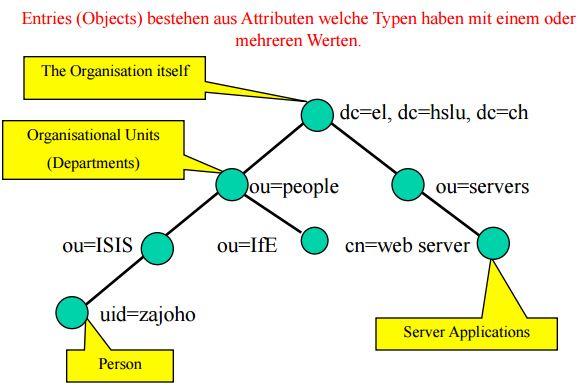
\includegraphics[width=0.6\linewidth]{fig/ldap-informations-modell}
\caption{Informations-Modell}
\label{fig:ldap-informations-modell}
\end{figure}

\subsubsection{Namens-Modell}
Die Datenstruktur ist ein hierarchischer Baum mit Wurzeln, Zweigen und Blättern. Dieser Baum wird auch Directory Information Tree (DIT) genannt. Die Wurzel (root, suffix) ist das oberste Datenobjekt, unter ihm verzweigen sich die höheren Strukturen. Oft wird der Unternehmensnamen als Wurzerl definiert \emph{o=css}. Personen können dann beispielsweise darunter angelegt werden \emph{ou=people,o=css} oder Gruppen \emph{ou=groups,o=css}. Ein einzelnes Objekt wird durch den Distinguished Name (DN) eindeutig identifiziert \emph{uid=tdsuter,ou=people,o=css}. Dieser setzt sich aus mehreren Relative Distinguished Names (RDN) zusammen. Eine anderen Namen für DN ist der canonical Namen, wobei der Pfad mit Slashes getrennt wird: \emph{css/people/tdsuter}. Oder an der HSLU: cn=Bruno Joho, ou=People, dc=el, dc=hslu, dc=ch. Einige bekannte Abkürzungen:

\begin{itemize}
	\item cn = common name
	\item ou = organizational unit
	\item st = state
	\item c = country
	\item mail = e-mail
	\item dc = domain component
\end{itemize}

\begin{figure}[h!]
\centering
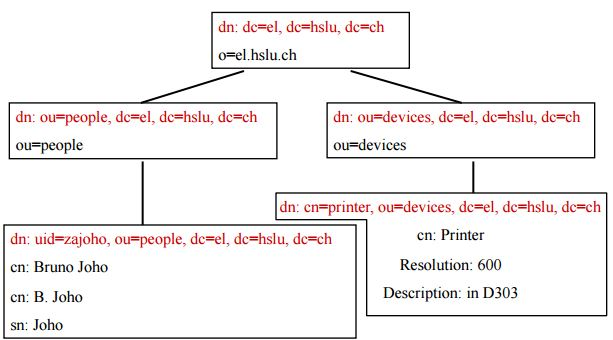
\includegraphics[width=0.7\linewidth]{fig/ldap-namens-modell}
\caption{Namens-Modell}
\label{fig:ldap-namens-modell}
\end{figure}

\subsubsection{Sicherheits-Modell}
Dieses Modell bietet eine flexible Zugriffskontrolle: Entire directory information tree (DIT), Sub-tree, Attribute level, User/Group und Authentication method. Zudem existieren Access Control-Instruction (ACI) \verb|aci = (targetattr != ‘userPassword’) (allowread,search,compare)| \\ \verb|(version 3.0; userdn=‘ldap:///anyone’;)|. Ausserdem kann natürlich entweder SSL oder TLS verwendet werden. Benutzt x.509 basierte Zertifikate. LDAP über SSL wird LDAPS abgekürzt.

\subsubsection{Funktionale-Modell}
Es gibt \textbf{interrogation Operationen}, welche zur Abfrage dienen. Es gibt keinen Read-Operator sondern nur einen Search, welcher bis zu 8 Parameter kennt. Dazu gibt es \textbf{Update-Operationen} (Hinzufügen, Löschen, Verändern). Zu guter letzt exsitieren die \textbf{Authentcation \& Control Operations} (Bind, Unbind, Abandon).

\subsubsection{Zugiff-Modell}
Neben den vier aufgelisteten Modellen, gibt es natürlich nun einfach noch ein fünftes. 
\begin{figure}[h!]
\centering
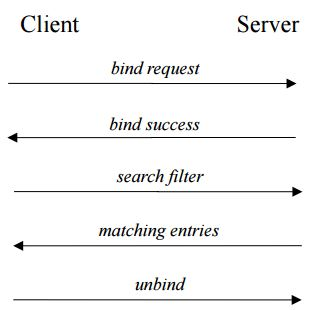
\includegraphics[width=0.4\linewidth]{fig/ldap-zugriffs-modell}
\caption{Zugriffs-Modell}
\label{fig:ldap-zugriffs-modell}
\end{figure}

\section{Kontrollfragen}

\subsection{Wie nennt man das Interface das die Gegenstelle zum API bildet und die eine problemlose Kommunikation mit dem Java API ermöglichen soll?}
SPI - Service Provider Interface. Das benötige ich, wenn ich den Service implementieren will. Wenn ich den Service verwenden will, benutze ich das API. Ein LDAP Server bietet ein SPI an, genauso wie ein API.

\subsection{Was ist LDAP? - MEP}
Lightweight Directory Access Protocol. Es ist ein Zugriffsprotokoll \& ein Directory Standard, da könnte man sagen, ja es ist mehr wie nur ein Protokoll. Es beinhaltet 4 Modelle.

\subsection{Wie würden Sie bei einem LDAP Daten austauschen?} 

Mittels dem LDIF Protokoll.

\subsection{Welche 2 Services stellt das JNDI zur Verfügung?}
\begin{description}
	\item[Namensdienst:] Mapping zwischen Namen und Objekt.
	\item[Verzeichnisdienst:] Erweiterter Namensdienst - zusätzliche Attribute pro Objekt.
\end{description}

\subsection{Was muss als allererstes erzeugt werden bei einer möglichen Verwendung eines Naming Services um ein Java Objekt zu registrieren?}
Heute verwende ich Dependency Injection um an JNDI-Ressourcen zu gelangen. Das kann ich technisch mit Annotationen (\verb|@EJB|) oder über den Deployment Deskriptor lösen. Trotzdem gibt es immer noch Fälle wo das ausprogrammiert werden muss. Falls ich das aber ausprogrammieren müsste, dann benötige ich den \textbf{Initial Context} (Wo finde ich was) sowie \textbf{Servername und Port}. Ich erzeuge mir also zuerst den Initial Context um danach eine Verbindung mit dem Verzeichnisdienst herzustellen. Für die Anfrage brauche ich natürlich noch den JNDI-Namen.

\subsection{Nennen Sie einige der Basismethoden mit denen Sie auf den Namensdienst zugreifen resp. navigieren?}
Folgende Methoden sind relevant: Bind, Lookup, Search, List, Unbind, Rebind, Add, Remove, Change. Wobei Joho folgende drei gerne hört: Lookup, List, Bind - diese sind LDAP spezifisch. Man bindet sich an einen Server.

\emph{Zusatzfrage: Wie wird denn im Gegensatz zu einer Datenbank eine LDAP Anfrage gemacht? - Eine Datenbank Anfrage macht man zuerst ein Open (wäre ein Bind), dann lassen sie diese offen (typischerweise im Applikationscontainer welche ein Pool von solchen Connections hat, weil diese teuer zu initialisieren sind, ganz im Gegensatz zum LDAP, der macht ein Bind und wenn er seine Antwort gekriegthat, gibt es ein unbind. Und dann wieder ein bind. Für jede Anfrage. Es wurde ja Entworfen für Telefonverzeichnisse, da wird sehr viel gelesen und nicht sehr viel geschrieben - ist leseoptimiert. Kann man nachlesen, wie viel mal schneller ein LDAP ist beim Lesen als eine Datenbank, dafür beim Schreiben naütrlich langsam.}

\subsection{Was ist ein distinguished Name (dn) und wie setzt er sich zusammen?}
Setzt sich aus dem Namen der Knoten zusammen - Sequenz von mehreren RDN (Relative Distinguished Name). Führt mich direkt zu einem Objekt (Knoten), dabei muss nicht erst die Verbindung geöffnet werden usw. Dann wird vom Objekt aus weiter gesucht oder man ist fertig. Man kann so die Suche sehr gut einschränken. \emph{(RDN = attribute:value)}

\emph{Wenn sie ein Distinguished Ingenieur sind - distinguished = ausgewählt - schenkt Joho einen Blumenstrauss. Ähnlich wie little endian (mail) und big endian (filesystem)}

\subsection{Welche 4 Modelle implementiert das LDAP Protokoll?}
\begin{itemize}
	\item Informationsmodell - Object Entries („Knoten“) in der Baumstruktur mit Attributen und Werten.
	\item Namensmodell - Jedes Object Entry ist über den dn eindeutig referenziert.
	\item Sicherheitsmodell - LDAP beinhaltet Interrogations Operations (Abfragen), Update Operations sowie Authentication and Control Operations.
	\item Funktionale Modell - Ermöglicht eine flexible Zugriffskontrolle auf die gesamte Baumstruktur, wobei die	Verbindung zum LDAP-Server über SSL / TLS zusätzlich noch abgesichert werden kann.
\end{itemize}

\subsection{Welche Operation nennt man Interrogation Operations (Abfrage) und welches Äquivalent hat sie in der Welt der Datenbanken?}
LDAP macht Search mit bis zu 8 Parameter, z.B. das Basisobjekt, der Search Scope (Einschränkung der Suche, hat seine Geschichte im Telefonbuch), Size Limit, Time Limit, Attribute-only Parameter, Filter, List Attribute von den Returnwerte - man kann direkt beim Search angeben, ich will nur 100 Einträge. In der DB ist es das Select im LDAP der Search.

\subsection{Was ist besonders an einer LDAP Anfrage, ganz im Gegensatz zu einer DB Anfrage?}
LDAP unterscheidet sich wesentlich im Lese- / Schreib-Verhältnis zu einer Datenbank: Durch die standardisierte \textit{baumartige} Struktur ist die Lesegeschwindigkeit (und nur diese!) wesentlich höher. Weiter kann die LDAP-Struktur nicht frei gewählt, sondern lediglich erweitert werden. LDAP ist zudem verteilbar und replizierbar. Die Verbindung wird nur für 1 Anfrage aufrecht erhalten, dann wird eine neue Verbindung gemacht. Man kann bestimmen wo im Verzeichnis die Suche beginnen soll. Bei der DB wird die Verbindung aufrechterhalten.